% !TeX root = ../main.tex
\chapter{Introduction}
\label{chapter:intro}

\section{Research Background and Significance}
\label{intro:sec:background}

Data centers serve as the "brains" of the Internet, providing the infrastructure necessary for storing vast amounts of data, performing large-scale computations, and offering Internet services. In the first decade of the 21st century, data centers primarily processed tasks that were easily parallelizable, such as websites and search engines. The rapid improvement in the performance of general-purpose processors also made the advantages of dedicated hardware less apparent. Consequently, Internet data centers often employed a large number of low-cost standard servers for construction \cite{barroso2009datacenter}.

In the past decade, the emergence of big data and artificial intelligence has altered the application load characteristics of data centers. On one hand, big data processing and machine learning workloads demand high computational power. However, due to the slowdown of Moore's Law and the end of Dennard's scaling law, the increase in frequency and number of multi-cores of general-purpose processors has been limited by the power wall in the past decade \cite{borkar2011future}. Therefore, the "free lunch" of general-purpose processor performance improvement has ended, ushering in the era of architectural innovation. Customized hardware such as GPUs, FPGAs, and TPUs \cite{jouppi2018motivation} are now widely deployed in data centers. On the other hand, big data processing and machine learning workloads require multiple nodes to work closely together, necessitating high inter-node communication bandwidth and low latency. To efficiently provide message passing and shared memory inter-process communication paradigms for distributed systems, efficient message passing needs to be implemented in the network, and high-performance shared data structure storage needs to be implemented at the storage level. Therefore, in the past decade, data center networks have evolved from 1 Gbps to 40 Gbps, and there is a trend to evolve to 100 Gbps. Dedicated interconnects between customized hardware are also becoming a trend. %As NVIDIA CEO Jensen Huang said, future data centers will be like supercomputers \cite{nvidia-datacenter}.

At the same time, the operational mode of data centers is also undergoing a transformation towards cloudification. A handful of cloud manufacturers are gradually centralizing the computing power of data centers, each possessing millions of servers. Due to the large scale of cloud data centers, cloud service providers can, on one hand, amortize the design and tape-out costs of servers, boards, and even chips, and on the other hand, improve performance indicators and reduce costs through software optimization, thereby achieving significant economic benefits. 

The cloudification of data centers means that a few cloud manufacturers maintain the basic infrastructure of data centers, and IT companies only need to rent computing, network, storage, and other resources from these cloud manufacturers as needed. In cloud data centers, different tenants share a vast pool of computing, storage, and network resources. To achieve resource sharing and performance isolation, data centers require virtualized computing, storage, and networks. 

As shown in Figure \ref{intro:fig:virt-architecture}, under the Infrastructure as a Service (IaaS) cloud service model, computing nodes need to provide services such as virtual networks, virtual cloud storage, and virtual local storage, while the actual network and cloud storage resources are located on independent network nodes and storage nodes. The virtual network and storage services on the computing nodes virtualize the physically dispersed network and storage resources in the data center into logically unified resources ("multi-virtual one"), akin to a large-scale computer \cite{barroso2018datacenter}. 

Network and storage nodes not only need to share physical resources with virtual machines of different tenants on multiple computing nodes ("one virtual multi"), but also need to provide data processing functions and high-level abstractions. For instance, network nodes need to provide \textit{network functions} such as firewalls, load balancing, encrypted tunnel gateways, and Network Address Translation (NAT)\footnote{In this article, \textit{network function} is a proper noun, not referring to network devices such as switches and routers, but referring to functions in network infrastructure such as firewalls.}; storage nodes need to perform data structure processing to provide high-level abstractions such as object storage and file system storage, and need to perform replication for disaster recovery.

In addition to persistent storage, data centers also need to provide memory data structure storage to support communication in distributed systems\footnote{Communication in distributed systems has two paradigms: message passing and shared memory. Message passing can be directly mapped to network communication. The shared memory paradigm is more developer-friendly, can support high availability and scalability, and needs to be implemented through message passing in distributed systems with network interconnection. However, the abstraction level of shared memory is relatively low, so most distributed systems use shared data structure storage to replace shared memory.}.
%Chapter \ref{chapter:background} will introduce the background knowledge of data center virtualization in detail.

\begin{figure}[htbp]
	\centering
	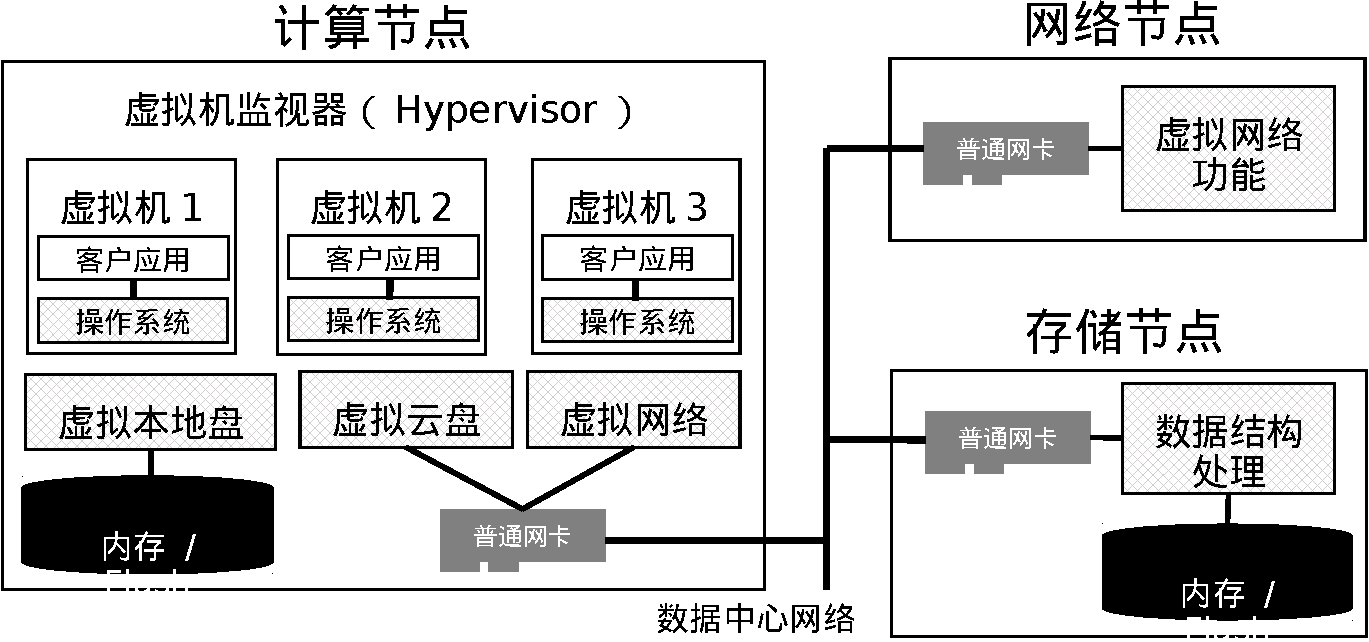
\includegraphics[width=0.8\textwidth]{figures/virt_arch.pdf}
	\caption{Virtualized data center architecture.}
	\label{intro:fig:virt-architecture}
\end{figure}

Due to the rapid evolution of cloud services, these virtualized network and storage functions also require flexibility, programmability, and debuggability, which are traditionally often implemented by software running on general-purpose processors. Besides virtualization overhead, the overhead of traditional operating systems cannot be overlooked. The software overhead depicted in the shadowed boxes in Figure \ref{intro:fig:virt-architecture} is referred to as the "data center tax" \cite{barroso2009datacenter,barroso2013datacenter,barroso2018datacenter}.
In the era of 1 Gbps networks and mechanical hard drives, the CPU overhead and latency introduced by network and storage virtualization as well as the operating system's network and storage protocol stack were acceptable.
With the trend of increasingly faster networks, storage, and customized computing hardware, the data center tax not only squanders significant CPU resources but also hinders applications from fully exploiting the low latency and high throughput of hardware \cite{barroso2017attack}.
For instance, as will be elucidated in Chapter \ref{chapter:clicknp}, computing nodes need to allocate a portion of the CPU cores specifically for implementing network and storage virtualization, and these cores will not be available for sale to customers.
Additionally, virtual networks and network functions will add tens to thousands of microseconds of latency. For comparison, the latency of the data center network itself is only a few to tens of microseconds, and the latency added by virtualization is higher than the latency of the network itself.
Chapter \ref{chapter:kvdirect} will explain that the throughput of software-implemented shared memory data structure storage is far from that of memory hardware.
%If you consider that the storage data needs to be compressed and encrypted, each CPU core can only process throughput on the order of 100 MB/s, which is only about 1/50 of the maximum throughput of a data center-level NVMe SSD.
Chapter \ref{chapter:socksdirect} will explain that applications generally use the socket primitives in the operating system for communication. For communication-intensive applications such as web servers, the operating system occupies a large part of the CPU time; moreover, the socket primitives implemented by the operating system have an order of magnitude higher latency than the Remote Direct Memory Access (RDMA) primitives provided by the hardware.

In summary, it is of great importance to reduce the "data center tax" through full-stack optimization combining hardware and software for the performance and cost of modern data centers, which is also the subject of this paper.

\section{Research Status at Home and Abroad}

In order to reduce the overhead of the "data center tax", the academic and industrial communities have proposed many solutions, which can be roughly divided into three categories: optimizing software, utilizing new commercial hardware, and designing new hardware.

\subsection{Optimizing Software}
\label{background:sec:software}

Traditional network functions are implemented by dedicated devices deployed in specific locations in the data center. These dedicated network function devices are not only expensive, but also not flexible enough to support multi-tenancy in cloud services. 
Therefore, cloud service providers have deployed software-implemented virtual network functions. For instance, Ananta \cite {ananta} is a software load balancer deployed in Microsoft data centers, used to provide cloud-scale load balancing services.
Works such as RouteBricks \cite {routebricks} demonstrate that the speed of each server forwarding packets based on multi-core x86 CPUs can reach 10 Gbps, and capacity can be expanded by multi-core and building more network node clusters.
Although software-implemented virtual switches and network functions can use a larger number of CPU cores and larger network node clusters to support higher performance, doing so will increase considerable asset and operating costs \cite {ananta,duet}.
The profitability of cloud service providers in IaaS business is the difference between the price paid by customers for virtual machines and the cost of hosting virtual machines.
Since the asset and operating costs of each server are basically determined at the time of deployment, the best way to reduce the cost of hosting virtual machines is to package more customer virtual machines on each computing node server and reduce the number of servers for network and storage nodes.
Currently, the price of a physical CPU core (2 hyperthreads, i.e., 2 vCPUs) is about \$0.1 per hour, i.e., the maximum potential income is about \$900 per year \cite{smartnic}.
In data centers, servers usually serve for 3 to 5 years, so the highest price of a physical CPU core during the server's life cycle can reach \$4500 \cite{smartnic}.
Even considering that some CPU cores are not sold out, and the cloud often offers discounts to large customers, compared with dedicated hardware, it is quite expensive to allocate a physical CPU core specifically for virtual networks.

Most applications access the network through the socket interface provided by the operating system. The sockets of existing operating systems such as Linux were designed for low-speed networks decades ago and have high overhead in today's high-throughput, low-latency data center networks.
In recent years, a lot of work has been devoted to providing high-performance sockets.
The first type of work is to optimize the TCP/IP network protocol stack of the operating system kernel.
However, a lot of kernel overhead still exists, which will be discussed in detail in Chapter \ref {chapter:socksdirect}.
The second type of work completely bypasses the kernel TCP/IP protocol stack and implements TCP/IP in user space, known as user-mode protocol stacks.
In this category, some works \cite {belay2017ix,peter2016arrakis} propose new operating system architectures, using virtualization to ensure security and isolation.
In addition to these new operating system architectures, many user-mode protocol stacks utilize high-performance packet I/O frameworks that already exist on Linux \cite {rizzo2012netmap,dpdk,pf-ring}.
Among them, some user-mode protocol stacks \cite {marinos2014network,jeong2014mtcp,seastar,fstack} believe that the Linux socket API is the root of performance overhead, and thus propose new APIs, which require modifying applications.
Most API changes aim to support zero copy.
Some other systems \cite {kalia2016fasst,kalia2018datacenter} go further, believing that the abstraction level of sockets is too low, and applications should use a higher-level remote procedure call (RPC) interface.
Since sockets are widely used, it is not realistic to require applications to modify the interface in many cases.
Therefore, some systems in the industry \cite{libvma,openonload,dbl} and academia \cite{huang2017high} propose user-mode TCP/IP protocol stacks that comply with the standard socket API.
These user-mode protocol stacks provide better performance than Linux, but they are still not close to the performance limit of hardware.
Currently, the performance benchmark for host-to-host communication in data center networks is Remote Direct Memory Access (RDMA), and the most efficient method for inter-process communication within a host is shared memory.
The host-to-host communication latency of these user-mode protocol stacks is an order of magnitude higher than RDMA, and the intra-host communication latency is one to two orders of magnitude higher than shared memory.

As a fundamental infrastructure for communication and storage in distributed systems, the exploration and advancement of Key-Value Storage systems have persistently been a primary concern in the academic and industrial systems community. The performance of early memory key-value storage systems \cite{memcached} was not satisfactory. Given that distributed systems are interconnected through networks, the user clients and storage servers of key-value storage systems also need to communicate through networks, introducing the overhead of socket network protocol stacks and network virtualization discussed earlier. 

To eliminate the overhead of the operating system kernel, recent key-value storage systems \cite {kapoor2012chronos,ousterhout2010case,ousterhout2015ramcloud,lim2014mica,li2016full} employ high-performance network packet processing frameworks, poll network packets from network cards, and utilize the aforementioned user-mode lightweight network protocol stacks to process them. However, even without considering the overhead of the network, the cost of key-value storage systems for data structure processing is also high. 

To reduce computing costs, a series of works \cite{mao2012cache,fan2013memc3,li2014algorithmic} optimize locks, caches, hashes, and memory allocation algorithms. To reduce the inter-core synchronization overhead of multiple CPU cores processing the same key, a more efficient method is for a fixed CPU core to handle each key's write operations \cite{lim2014mica}. 

However, due to the limitations of CPU parallelism, as will be discussed in Chapter \ref{chapter:kvdirect}, even if optimized to the extreme, each CPU core can only handle about 5 million key-value operation requests per second, far lower than the hardware performance that memory random access can provide. 

In addition, the keys in real-world workloads often follow a long-tail distribution, that is, a small number of keys are accessed very frequently, and most keys are not frequently accessed. Under long-tail distribution loads, because the same key is always mapped to the same CPU core, it will lead to load imbalance among CPU cores \cite{lim2014mica}.

\subsection{Utilizing New Commercial Hardware}

Due to the pressing performance demands of large-scale web services, big data processing, machine learning, and other computing and networking applications, computing acceleration devices such as Graphics Processing Units (GPUs) and network acceleration technologies such as Remote Direct Memory Access (RDMA) \cite{infiniband2000infiniband} are increasingly being deployed in data centers.

To speed up virtual networks and network functions, previous research has suggested the use of GPUs \cite{packetshader}, Network Processors (NPs) \cite{cavium,netronome}, and hardware network switches \footnote{In this paper, the term \textit{switch} is used interchangeably with router, and the term \textit{switch} is commonly used in data center-related literature to refer to network interconnection devices.} \cite{duet}. GPUs were initially used primarily for graphics processing, but in recent years have been extended to other applications with massive data parallelism. GPUs are suitable for batch operations, but batch operations can lead to high latency. The history of network processors can be traced back to network switches of the 1990s. Network processors consist of a large number of embedded processor cores, each with limited processing power, and stateful connections are usually handled by fixed processor cores, thus limiting the throughput of a single connection. The main problem with hardware network switches is their lack of flexibility and insufficient lookup table capacity \cite{duet}.

To reduce the overhead of operating system communication primitives, a series of work has offloaded \footnote{In this paper, \textit{offload} is a term that refers to implementing functions that are implemented in software on the host CPU using hardware other than the host CPU.} part of the operating system network protocol stack to network card hardware. The TCP Offload Engine (TOE) \cite{tcp-chimney-offload} offloads part or all of the TCP/IP protocol stack to the network card. However, due to the rapid growth of general-purpose processor performance according to Moore's Law, the performance advantages of these dedicated hardware are limited and have only been successful in dedicated fields. The commercially successful TCP offload functions are mostly stateless offloads \footnote{\textit{Stateless} means that the internal storage of the network card is read-only during packet processing.}, such as offloading of TCP checksums. Infiniband \cite{infiniband2000infiniband} technology designed a new set of communication primitives, transport layer protocols, network layer protocols, and physical transmission media. The communication primitives and transport layer protocols are known as Remote Direct Memory Access (RDMA). Infiniband implements the entire network protocol stack in hardware, achieving high throughput and low latency, and is widely used in the field of high-performance computing. Since the transport layer needs to maintain the state of each connection to implement congestion control, packet retransmission, out-of-order rearrangement, etc., Infiniband is a stateful offload. In recent years, due to the hardware trends and application requirements of data centers, the story of stateful offload has begun to revive \cite{chuanxiong-rdma-keynote}. RDMA based on Infiniband technology is widely deployed in data centers \cite{guo2016rdma}. In order to be compatible with the existing Ethernet in data centers, data centers do not use Infiniband physical layer networks, but strip the RDMA primitives and transport layer protocols from the Infiniband technology stack, encapsulate RDMA transport layer packets in UDP/IP packets, and transmit them through Ethernet, which is called RoCEv2 \cite{rocev2}. Compared with the software-based TCP/IP network protocol stack, RDMA uses hardware offloading to provide ultra-low latency and near-zero CPU overhead.

RDMA communication primitives significantly differ from the socket communication primitives typically used by applications. RDMA is message-based, whereas sockets are stream-based. RDMA necessitates applications to explicitly register and manage send and receive buffers. It also requires applications to manage send, receive, and event queues, and to timely send flow control notifications to the network card. RDMA offers two types of communication primitives. The first type is two-sided operations, similar to sockets, where the sender calls send and the receiver calls recv. Unlike sockets, the RDMA receiver application needs to predeclare the messages to be received and prepare the receive buffer for the network card. The other type is one-sided operations, which provide shared memory primitives, i.e., direct read and write of remote memory, or atomic operations on remote memory. Consequently, RDMA programming is considerably more complex than socket programming. An example program that sends and receives with sockets requires only a few dozen lines of code, while the same functionality with RDMA requires hundreds of lines of code. To enable socket applications to use RDMA, works like RSocket \cite{rsockets,socketsdirect,russell2008extended} convert socket operations into RDMA primitives. They have similar designs, with RSocket being the most actively developed and the de facto standard for converting sockets to RDMA. However, the performance and compatibility of RSocket are not satisfactory. Chapter \ref{chapter:socksdirect} will propose a socket system that is compatible with existing applications and can fully utilize the performance of RDMA network cards.

In addition to network communication between hosts, inter-process communication within a host is also crucial. Some work \cite {belay2017ix,peter2016arrakis,rsockets} allows inter-process communication within a host to bypass the RDMA network card. However, due to the limitations of the PCIe bus, the latency and throughput of the RDMA network card are much worse than the shared memory within the host. Therefore, Chapter \ref{chapter:socksdirect} uses shared memory to implement inter-process communication within the host.

To enhance the performance of key-value storage systems, recent research \cite {kalia2014using,kalia2016design,kalia2014using,kalia2016design} has utilized the hardware-based network protocol stack of the RDMA network card. This approach uses bilateral RDMA as the remote procedure call mechanism between the key-value storage client and server, thereby significantly increasing per-core throughput and reducing latency, as illustrated in Figure \ref{intro:fig:memaccess-a}. Although these studies have further reduced the overhead of network communication, as discussed in Section \ref{background:sec:software}, these systems still rely on the server-side CPU for data structure processing, which hampers performance.

\begin{figure*}[t]
	\centering
	\subfloat[Software / Bilateral RDMA.\label{intro:fig:memaccess-a}]
	{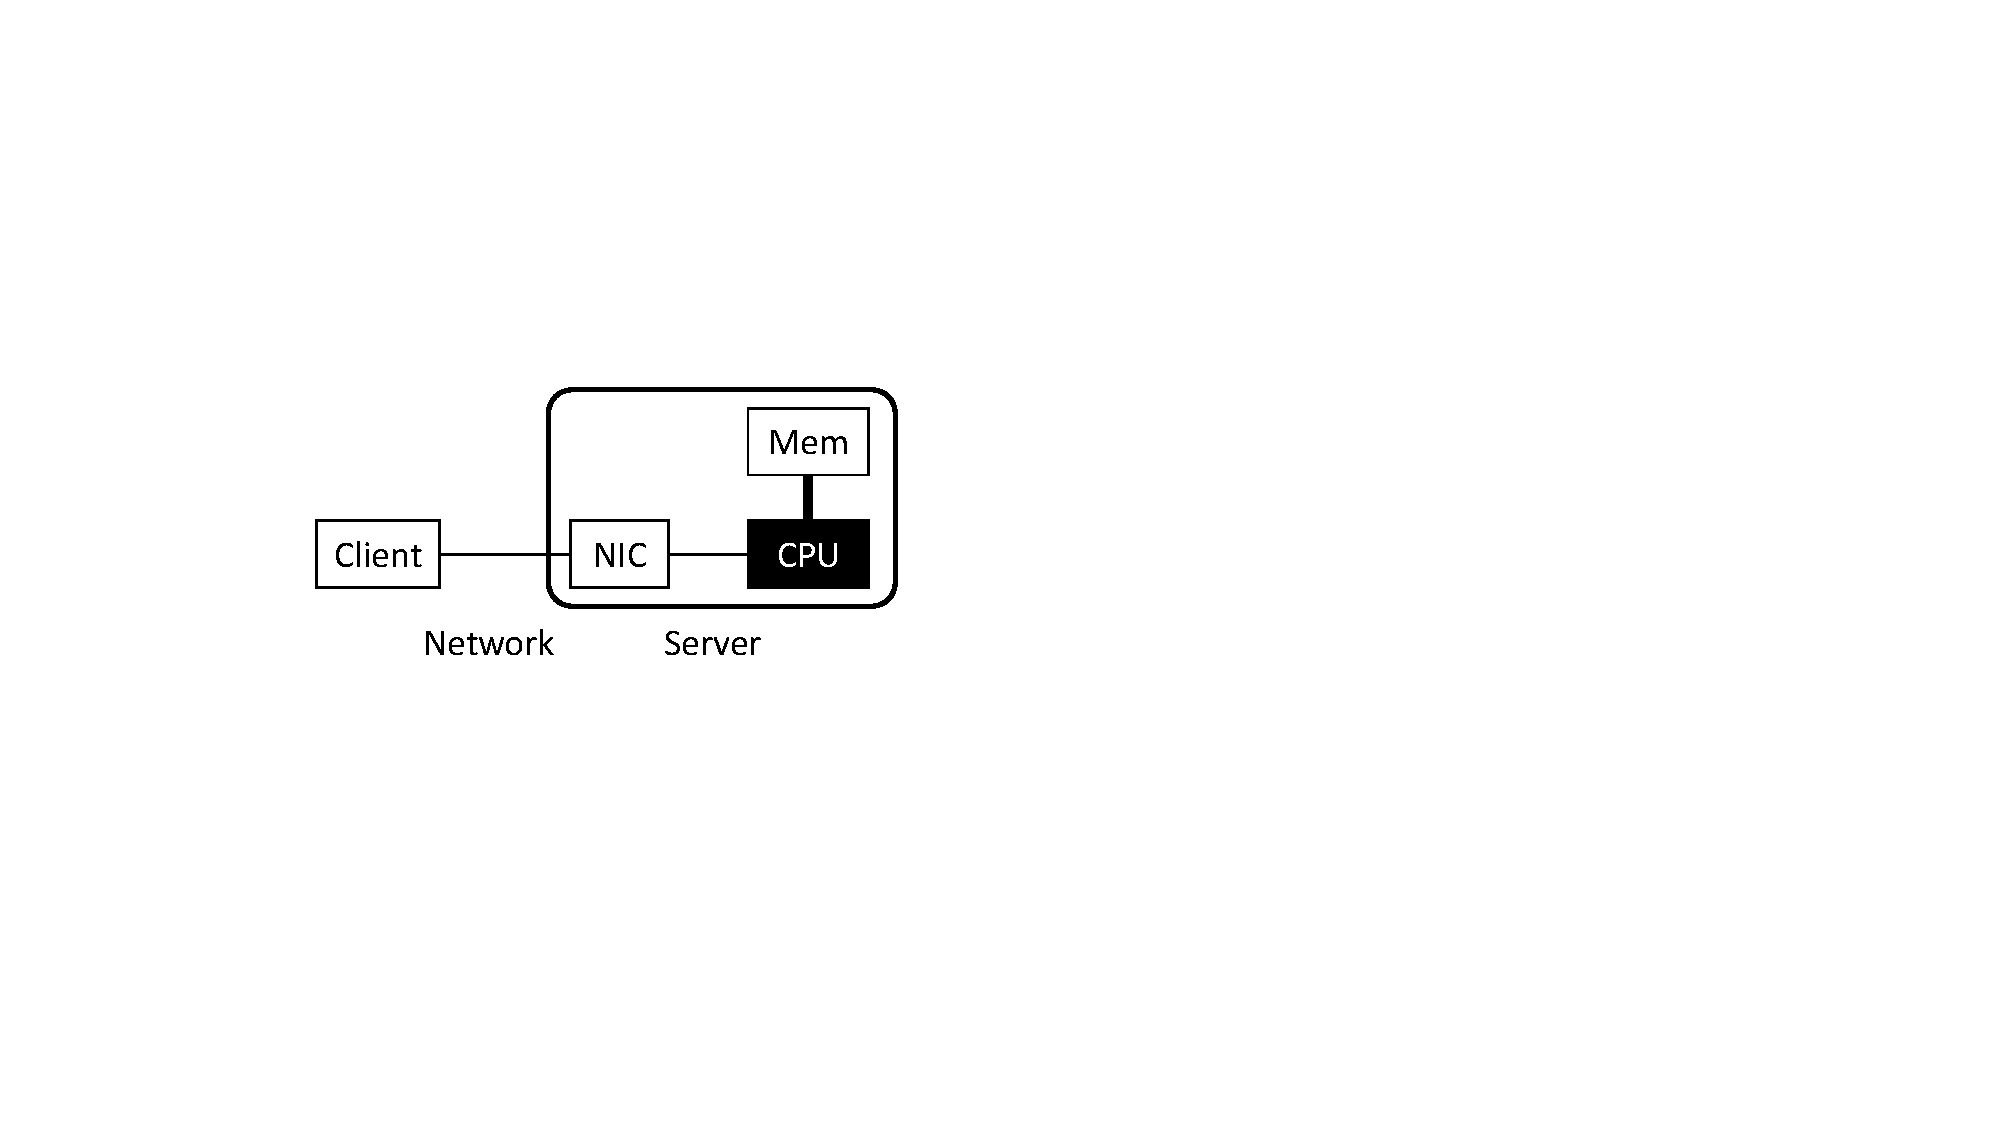
\includegraphics[width=.4\textwidth,page=1]{cropped_access.pdf}}
	\subfloat[Unilateral RDMA.\label{intro:fig:kvdirect-b}]
	{\includegraphics[width=.4\textwidth,page=2]{cropped_access.pdf}}
	\caption{Architecture of key-value storage systems. Lines represent data paths. A key-value operation (thin line) may require multiple address-based memory accesses (thick line). The box with a black background indicates where key-value data structure processing occurs.}
	\label{intro:fig:kvdirect}
\end{figure*}

An alternative strategy is to employ unilateral RDMA, which shifts the data structure processing of the server-side CPU to the client, as shown in Figure \ref{intro:fig:kvdirect-b}. The client initiates read and write requests to the server-side shared memory via unilateral RDMA, and the server-side network card directly accesses the memory without involving the CPU. However, using shared memory mode to access data structures often necessitates multiple network round trips (for instance, querying the index first and then accessing the data), which increases access latency and consumes network bandwidth. Moreover, this mode is not suitable for write-intensive workloads. When multiple clients attempt to manipulate the same data structure (for example, allocating memory or modifying the same key-value pair), they must lock or synchronize between clients, which introduces additional latency and bandwidth overhead.

\subsection{Designing New Hardware}

As the performance improvement of general-purpose processors has hit a wall, major cloud service providers have started to explore the use of custom hardware to reduce the "data center tax". This means shifting the overhead of data center virtualization, operating systems, and high-level abstractions from general-purpose processors to custom hardware. The use of custom hardware is not about implementing existing software in hardware as it is, but rather refactoring existing software, dividing it into a data plane and a control plane, optimizing the data plane and implementing it in hardware, and leaving the control plane in software. Although the solution using new hardware has higher performance, it requires not only the assets and operating costs of new hardware, but also the development costs of software and hardware co-design, which are often higher than the one-time research and development (Non-Recurring Engineering, NRE) cost of simply optimizing software. In addition, compared to developing and testing software, designing, verifying, and mass-producing new hardware requires a longer R\&D cycle. Programmable hardware has a certain degree of flexibility, but it is limited compared to general-purpose processors, so it requires a certain foresight of future data center application loads and infrastructure. Therefore, not all software is suitable for hardware acceleration, and it is necessary to weigh multiple factors such as cost, benefit, R\&D cycle, and flexibility. Due to the massive scale of cloud services, the overhead of the "data center tax" is also widespread and significant, so it is worth designing programmable hardware for acceleration.

To minimize the CPU cores used for virtual networks on computing nodes, cloud service providers, represented by Microsoft Azure, have deployed a programmable network card on each server in the data center to accelerate virtual networks \cite{smartnic}. To provide high performance while maintaining a certain degree of programmability and flexibility, the industry has proposed programmable network card architectures such as dedicated chips (ASIC), network processors (Network Processor), multi-core general-purpose processor system-on-chip (SoC), and field-programmable gate arrays (FPGA), which will be discussed in detail in Section \ref{smartnic-architecture}. FPGA achieves a balance between performance and flexibility, so Microsoft uses an FPGA-based programmable network card \cite{putnam2014reconfigurable}.

FPGAs have been extensively utilized in the implementation of network routers and switches. However, FPGAs are typically programmed in hardware description languages such as Verilog and VHDL. As is widely recognized, hardware description languages are challenging to debug, write, and modify, which presents a significant obstacle for software personnel to utilize FPGAs. To enhance the development efficiency of FPGAs, FPGA manufacturers offer high-level synthesis (HLS) tools~\cite{vivado,intel-hls} capable of compiling restricted C code into hardware modules. However, these tools merely supplement the hardware development toolchain. Programmers still need to manually insert the hardware modules generated from C language into the hardware description language project, and they must handle the communication between the FPGA and the host CPU themselves. The academic and industrial communities have proposed efficient hardware development languages such as Bluespec \cite{bluespec}, Lime \cite{auerbach2010lime}, and Chisel \cite{bachrach2012chisel} \cite{bacon2013fpga,singh2011implementing,wester2015transformation}, but these require developers to possess substantial hardware design knowledge. High-level synthesis tools and efficient hardware development languages can enhance the work efficiency of hardware developers, but they are still insufficient for software developers to utilize FPGAs.

In recent years, to enable software developers to use FPGA, FPGA manufacturers have proposed OpenCL-based programming toolchains~\cite{aoc,sdaccel}, providing a GPU-like programming model. Software developers can offload kernels written in OpenCL language to FPGA. However, in this method, multiple parallelly executing kernels need to communicate through shared memory on the board, and the throughput and latency of DRAM shared memory on FPGA are not ideal, and shared memory can become a communication bottleneck. Secondly, the communication model between FPGA and CPU is similar to the GPU's batch processing model, which results in higher processing latency (about 1 millisecond), which is not suitable for network packet processing that requires microsecond-level latency.
Chapter \ref{chapter:clicknp} of this paper will propose a modular FPGA programming framework that is available to software developers and has high performance for network packet processing.
Based on this, Chapter \ref{chapter:kvdirect} will use programmable network cards to extend the shared memory read and write primitives of RDMA to key-value operation primitives, and use programmable network cards to implement high-throughput, low-latency memory key-value storage.

\section{Research Content and Contributions of This Paper}

This paper aims to explore high-performance data center systems that are constructed on programmable network cards. It presents a system that enhances the full stack of computing, networking, and storage nodes in cloud computing data centers, utilizing FPGA programmable network cards. As illustrated in Figure \ref{intro:fig:accel-arch}, by replacing the standard network cards on the computing, networking, and storage nodes with programmable network cards, this paper implements virtual network cards and virtual networks, virtual local storage and cloud storage, and lightweight user-state runtime libraries on the computing nodes. Furthermore, the integration of hardware transport protocol communication primitives supplants the software virtualization services and operating system network protocol stack in Figure \ref{intro:fig:virt-architecture}. This paper also implements the virtual network functions of network nodes and the memory data structure processing of storage nodes based on the concept of separating the data plane and the control plane, enhances the data plane performance with programmable network cards, and retains the flexibility of the original software control plane.

\begin{figure}[htbp]
	\centering
	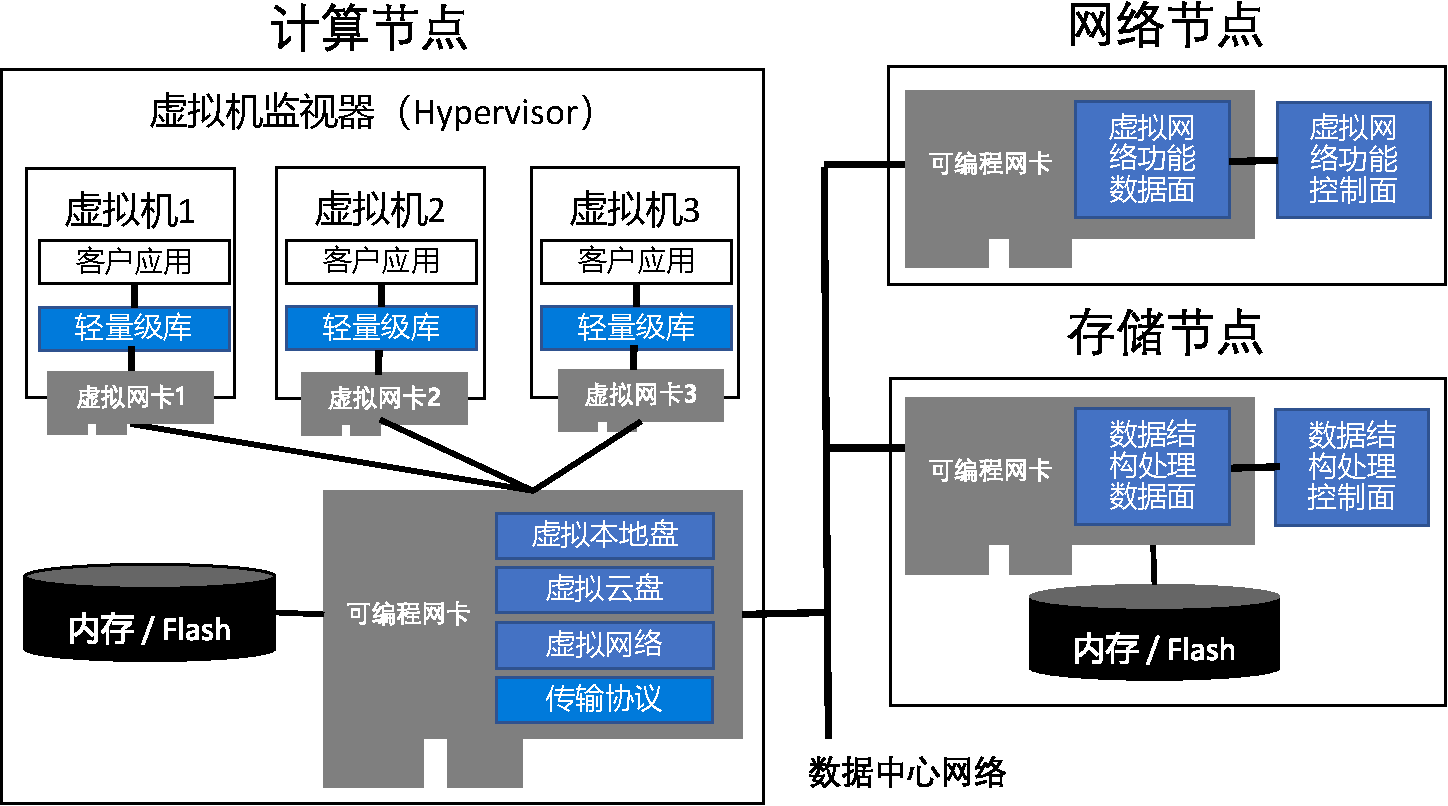
\includegraphics[width=0.8\textwidth]{figures/accel_arch.pdf}
	\caption{Overall architecture of the data center system based on programmable network cards.}
	\label{intro:fig:accel-arch}
\end{figure}

Firstly, this paper proposes to accelerate the virtual network functions in cloud computing with programmable network cards. It introduces the first high-flexibility, high-performance network function processing platform ClickNP, accelerated by FPGA in commercial servers. It is well known that FPGA programming is not user-friendly for software engineers. To simplify FPGA programming, a C-like ClickNP language and a modular programming model are designed, and a series of optimization techniques are developed to fully exploit the massive parallelism of FPGA. The ClickNP development toolchain is implemented, which can be integrated with various commercial high-level synthesis tools. More than 200 network elements are designed and implemented based on ClickNP, and these elements are used to construct various network functions. Compared with CPU-based software network functions, ClickNP's throughput is increased by 10 times, and the latency is reduced to 1/10; and it has negligible CPU overhead, which can save 20\% of CPU cores for each computing node in cloud computing.

Secondly, this paper presents a method to accelerate access to remote data structures using programmable network cards. Key-value storage, a fundamental data structure often used, plays a crucial role in numerous distributed systems within data centers. A high-performance memory key-value storage system, KV-Direct, is developed based on the ClickNP programming framework. This system bypasses the server-side CPU and utilizes programmable network cards to directly access the host memory via PCIe. The memory operation semantics of one-sided RDMA are extended to key-value operation semantics, addressing the high communication and synchronization overhead when one-sided RDMA operates data structures. The reconfigurable feature of FPGA is also utilized, allowing users to implement more complex data structures. To address the performance challenges of lower PCIe bandwidth and higher latency between the network card and the host memory, a series of performance optimizations are employed, such as hash tables, memory allocators, out-of-order execution engines, load balancing and caching, vector operations, etc. These optimizations enable 10 times the energy efficiency of the CPU and microsecond-level latency, and for the first time, single-machine performance reaches 1 billion operations per second in a general key-value storage system.

Lastly, this paper presents a method that integrates programmable network cards and user-state runtime libraries to provide system primitives for applications, thereby bypassing the operating system kernel. The socket, the most commonly used communication primitive provided by the operating system, is redesigned and implemented in a user-state socket system, SocksDirect. This system is fully compatible with existing applications, can achieve throughput and latency close to hardware limits, has scalable multi-core performance, and maintains high performance under high concurrent loads. Intra-host and inter-host communications are implemented using shared memory and RDMA respectively. To support a high number of concurrent connections, an RDMA programmable network card is implemented based on KV-Direct. By eliminating a series of overheads such as inter-thread synchronization, buffer management, large data copying, process awakening, etc., SocksDirect increases the throughput by 7 to 20 times compared to Linux, reduces the latency to 1/17 to 1/35, and reduces the HTTP latency of the web server to 1/5.5.

\section{Arrangement of Thesis Structure}

The structure of this thesis is organized as follows:
Chapter 1 serves as the introduction.
Chapter 2 presents the development trends of data centers, emphasizes the needs and opportunities for software and hardware co-optimization in data centers, discusses the architecture of programmable network cards, and reviews the application of programmable network cards in data centers.
Chapter 3 proposes a data center system architecture that is based on programmable network cards.
Chapter 4 is the network function acceleration section, suggesting the acceleration of virtual network functions in cloud computing using programmable network cards. To simplify FPGA programming, the first modular FPGA programming framework ClickNP, which is suitable for high-speed network packet processing and based on high-level languages, is proposed.
Chapter 5 is the data structure acceleration section, suggesting the acceleration of remote data structure access using programmable network cards, and designing and implementing a high-performance memory key-value storage system KV-Direct.
Chapter 6 is the operating system acceleration section, suggesting a method of integrating programmable network cards and user-state runtime libraries to provide system primitives for applications, and designing and implementing a user-state socket system SocksDirect.
Chapter 7 summarizes the entire text and anticipates future research directions.
